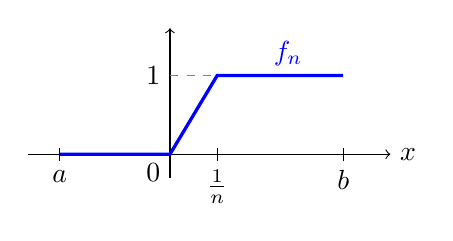
\begin{tikzpicture}
  \draw[->] (-1.8,0) -- (2.8,0) node[right] {$x$};
  \draw[->] (0,-0.3) -- (0,1.6);
  \draw[blue, very thick] (-1.4,0) -- (0,0) -- (0.6,1) -- (2.2,1);
  \draw[dashed, gray] (0,1) node[left, black] {$1$} -- (0.6,1);
  \draw (-1.4,0.08) -- (-1.4,-0.08) node[below] {$a$};
  \draw (0.6,0.08) -- (0.6,-0.08) node[below] {$\frac1n$};
  \draw (2.2,0.08) -- (2.2,-0.08) node[below] {$b$};
  \node[below left] at (0,0) {$0$};
  \node[blue, above] at (1.5,1) {$f_n$};
\end{tikzpicture}
